\documentclass[12pt]{article}

\usepackage[margin=1in]{geometry}
\usepackage{amsmath,amsthm,amssymb}
\usepackage{nccmath}
\usepackage{mathtools}
\usepackage{mathrsfs}
\usepackage{enumitem}
\usepackage{physics}
\usepackage{slashed}
\usepackage{pdfpages}
\usepackage{float}

\usepackage{tikz}
\usepackage{tikz-feynman}

\newcommand{\magsq}[1]{\big|#1\big|^2}

\begin{document}

\title{Homework 6}
\author{Sean Ericson \\ Phys 663}
\maketitle

\section*{Problem 1}
\begin{enumerate}[label=(\alph*)]
    \item Symmetrizing under $\epsilon_1 \leftrightarrow \epsilon_2$ and $\epsilon_4 \leftrightarrow \epsilon_3$, we get
    \[ \mathcal{M} \to a\left(\vec{\epsilon}_1\cdot\vec{\epsilon}_2\right)\left(\vec{\epsilon}_3^*\cdot\vec{\epsilon}_4^*\right) + \frac{b+c}{2}\left[\left(\vec{\epsilon}_1\cdot\vec{\epsilon}_3^*\right)\left(\vec{\epsilon}_2\cdot\vec{\epsilon}_4^*\right) + \left(\vec{\epsilon}_1\cdot\vec{\epsilon}_4^*\right)\left(\vec{\epsilon}_2\cdot\vec{\epsilon}_3^*\right)\right], \]
    which implies $b = c$, and we get two independent terms
    \begin{align*}
        \mathcal{M}_0 &\propto \left(\vec{\epsilon}_1\cdot\vec{\epsilon}_2\right)\left(\vec{\epsilon}_3^*\cdot\vec{\epsilon}_4^*\right) \\
        \mathcal{M}_> &\propto \left(\vec{\epsilon}_1\cdot\vec{\epsilon}_3^*\right)\left(\vec{\epsilon}_2\cdot\vec{\epsilon}_4^*\right) + \left(\vec{\epsilon}_1\cdot\vec{\epsilon}_4^*\right)\left(\vec{\epsilon}_2\cdot\vec{\epsilon}_3^*\right).
    \end{align*}

    \item In the center of mass frame, the momenta are
    \begin{align*}
        &p_1 = \frac{m_h}{2}(1, 0, 0, 1) && p_3 = \frac{m_h}{2}(1, \sin\theta, 0, \cos\theta) \\
        &p_2 = \frac{m_h}{2}(1, 0, 0, -1) && p_4 = \frac{m_h}{2}(1, -\sin\theta, 0, -\cos\theta)
    \end{align*}
    For spin-0 Higgs, by conservation of angular momentum the particles in the in state must have equal helicities (and similarly for the out state), while a spin-2 Higgs places no such restriction. For the matrix element $\mathcal{M}(g_+g_+ \to h \to \gamma_+\gamma_+)$, where the gluons and photons all have helicity $+1$, we have
    \begin{align*}
        &\vec{\epsilon}_1 = \frac{1}{\sqrt{2}}\mqty(1\\i\\0), & \vec{\epsilon}_3 = \frac{1}{\sqrt{2}}\mqty(\cos\theta\\i\\-\sin\theta), \\
        &\vec{\epsilon}_2 = \frac{1}{\sqrt{2}}\mqty(1\\-i\\0), & \vec{\epsilon}_4 = \frac{1}{\sqrt{2}}\mqty(-\cos\theta\\i\\\sin\theta).
    \end{align*}
    The relevant dot products are then
    \begin{align*}
        \vec{\epsilon}_1\cdot\vec{\epsilon}_2 &= 1 \\
        \vec{\epsilon}_3^*\cdot\vec{\epsilon}_4^* &= -1 \\
        \vec{\epsilon}_1\cdot\vec{\epsilon}_3^* = -\vec{\epsilon}_2\cdot\vec{\epsilon}_4^* &= \frac{1}{2}(\cos\theta + 1) \\
        \vec{\epsilon}_2\cdot\vec{\epsilon}_3^* = -\vec{\epsilon}_1\cdot\vec{\epsilon}_4^* &= \frac{1}{2}(\cos\theta - 1)
    \end{align*}
    Clearly, the first independent matrix element, $\mathcal{M}_0$, does not depend on $\theta$, as is appropriate for a spin-0 Higgs. Meanwhile, in this spin configuration, the second term is $\theta$-dependent but non-vanishing.
    \[ \mathcal{M}_> \propto \left(\cos\theta + 1\right)^2 + \left(\cos\theta - 1\right)^2 > 0 \]
    This is consistent with a spin-2 Higgs with 0 $z$-component spin projection (i.e. $j = 2,\; m = 0$)
    For the matrix element $\mathcal{M}(g_+g_- \to h \to \gamma_+\gamma_-)$, the polarization vectors are given by
    \[ \vec{\epsilon}_1 = \vec{\epsilon}_2 = \mqty(1\\i\\0), \]
    \[ \vec{\epsilon}_3 = \vec{\epsilon}_4 = \mqty(\cos\theta\\i\\-\sin\theta). \]
    Clearly, the spin-0 component vanishes (both dot products are zero), while 
    \[ M_> \propto \sin^2\theta, \]
    so the photons can't come out in the exact same orientation as the gluons came in.

    \item If we have a levi-civita fully contracted with the polarizations,
    \[ \epsilon_{\mu\nu\rho\sigma}\epsilon_1^\mu\epsilon_2^\nu\epsilon_3^\rho\epsilon_4^\sigma, \]
    symmetrization with respect to any two indices will vanish (due to the antisymmetry of the levi-civita), but we need to symmetrize w.r.t $1\leftrightarrow2$ and $3\leftrightarrow4$.

\end{enumerate}

\section*{Problem 2}
\begin{enumerate}[label=(\alph*)]
    \item 
    \begin{align*}
        V &= m_1^2\magsq{H_1} + m_2^2\magsq{H_2} - b(H_1^\dag H_2 + H_2^\dag H_1) + \frac{g^2 + g'^2}{8}\left(\magsq{H_1}-\magsq{H_2}\right)^2 + \frac{g^2}{2}\left(H_2^\intercal\epsilon H_1\right)\left(H_2^\dag\epsilon H_1^*\right) \\
        &= m_1^2\left(\magsq{H_1^+} + \magsq{H_1^-}\right) + m_2^2\left(\magsq{H_2^+} + \magsq{H_2^-}\right) - 2b\Re[H_1^{+*}H_2^+ + H_1^{-*}H_2^{-}] \\
        &\quad + \frac{g^2 + g'^2}{8}\left(\magsq{H_1^+} + \magsq{H_1^-} - \magsq{H_2^+} - \magsq{H_2^-}\right)^2 + \frac{g^2}{2}\magsq{H_1^+H_2^- - H_1^-H_2^+}
    \end{align*}
    Given that
    \begin{align*}
        \pdv{V}{H_1^+}\bigr\lvert_{H_1 = \left<H_1\right>, H_2 = \left<H_2\right>} &= -\frac{y^*}{4}\left(4b + \sqrt{2}g^2vz\right),
    \end{align*}
    we can see that $y=0$ gives a minimum of the potential.

    \item 
    \begin{align*}
        V\bigr\lvert_{H_1^+\to0,\;H_2^+\to0,;H_1^-\to v/\sqrt{2}} &= 
    \end{align*}
    For any complex value of $H_2^-$, keeping the magnitude fixed while rotating the number towards the positive real axis will decrease the value of the potential. Therefore, at the minimum of the potential $H_2^-$ must lie on the positive real axis.

    \item 
    \begin{align*}
        V &= m_1^2\left(\magsq{H_1^+} + \frac{1}{2}\magsq{v_1 + h_1 + iA_1}\right) + m_2^2\left(\magsq{H_2^+} + \frac{1}{2}\magsq{v_2 + h_2 + iA_2}\right) \\
        &\quad - 2b\Re[H_1^{+*}H_2^+] - b\left[(v_1+h_1)(v_2 + h_2) + A_1A_2\right] \\
        &\quad + \frac{g^2 + g'^2}{8}\left(\magsq{H_1^+} + \magsq{v_1 + h_1 + iA_1} - \magsq{H_2^+} - \magsq{v_2 + h_2 + iA_2}\right)^2 \\
        &\quad + \frac{g^2}{4}\magsq{H_1^+\left(v_2 + h_2 + iA_2\right) - \left(v_1 + h_1 + iA_1\right)H_2^+} 
    \end{align*}

    \begin{align*}
        \pdv{V}{h_1}\bigr\lvert_{H_1\to\left<H_1\right>,\;H_2\to\left<H_2\right>} &= v_1m_1^2 -bv_2 + \frac{1}{8}(g^2 + g'^2)v_1(v_1^2 - v_2^2) = 0 \\
        \implies m_1^2 &= b\frac{v_1}{v_2} - \frac{1}{8}(g^2 + g'^2)(v_1^2 - v_2^2)
    \end{align*}
    \begin{align*}
        \pdv{V}{h_2}\bigr\lvert_{H_1\to\left<H_1\right>,\;H_2\to\left<H_2\right>} &= v_2m_2^2 - bv_1 + \frac{1}{8}(g^2 + g'^2)v_2(v_2^2 - v_1^2) = 0 \\
        \implies m_2^2 &= b\frac{v_2}{v_1} - \frac{1}{8}(g^2 + g'^2)(v_2^2 - v_1^2)
    \end{align*}

    \item See Mathematica printout
    \item See Mathematica printout
    \item See Mathematica printout
\end{enumerate}

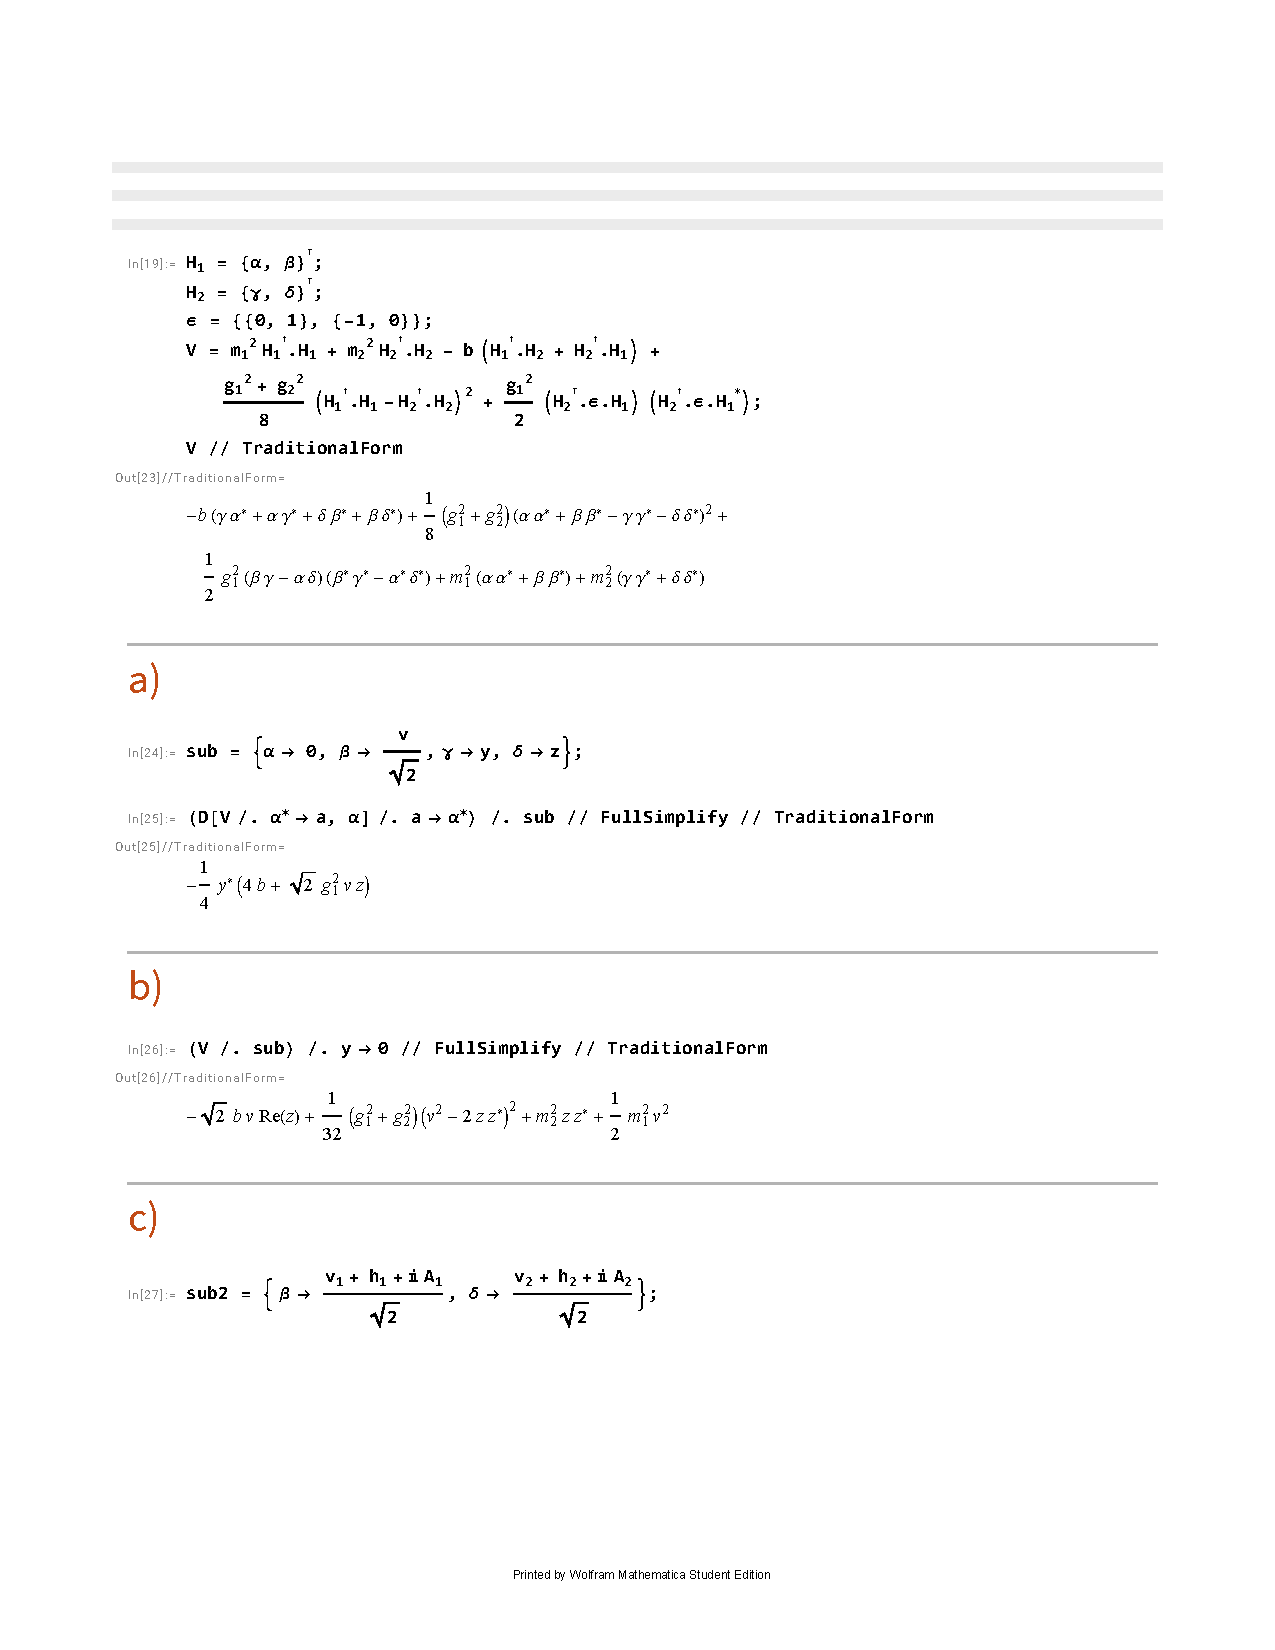
\includepdf[pages=-]{calcs/prob2.pdf}

\end{document}